\documentclass[12pt]{article}

\usepackage{etoolbox}
\usepackage{sbc-template}
\usepackage{graphicx,url}
\usepackage[utf8]{inputenc}
\usepackage[brazil]{babel}
\usepackage[none]{hyphenat}

\makeatletter
\patchcmd{\@startsection}
{\@afterindentfalse}
{\@afterindenttrue}
{}{}
\makeatother
     
\sloppy

\title{Análise da Localização Ótima de Farmácias no\\ Bairro Centro, Aracaju: Estudo de Caso}

\author{Anthony França, Antônio Neto, Enzo Santana, Franck Vasconcelos,\\
Murilo Mota, Rafael Gonçalves, Rene Marinho}

\address{Universidade Tiradentes (UNIT)\\}

\begin{document} 

\maketitle

     
\begin{resumo} 
O objetivo deste estudo é identificar a localização otimizada para farmácias no bairro Centro, em Aracaju, considerando fatores geográficos, econômicos e logísticos. Buscamos determinar áreas com melhor relevo, proximidade de comércio e distribuidores de medicamentos e infraestrutura adequada para operação. Farmácias já existentes serão desconsideradas, permitindo encontrar novas geolocalizações estratégicas. Além disso, serão analisadas regiões que já possuem outras empresas, possibilitando identificar terrenos disponíveis para locação ou compra, com potencial para instalação de farmácias. A abordagem combina critérios de acessibilidade, visibilidade e conveniência para clientes, visando maximizar eficiência operacional e cobertura de mercado. Os resultados fornecerão uma base prática para planejamento urbano e expansão do setor farmacêutico no bairro.
\end{resumo}


\section{Introdução}

A localização de estabelecimentos comerciais desempenha papel fundamental no desempenho e na sustentabilidade de negócios. No setor farmacêutico, esse aspecto torna-se ainda mais relevante, pois envolve não apenas critérios de competitividade, mas também de acesso à saúde e bem-estar da população. A escolha inadequada do ponto de instalação pode resultar em altos custos, baixa atratividade de clientes e dificuldades logísticas no abastecimento de medicamentos.

No contexto de Aracaju, especificamente no bairro Centro, observa-se uma concentração significativa de atividades comerciais e serviços. Trata-se de uma região com fluxo intenso de pessoas, proximidade de órgãos públicos e presença de distribuidores de medicamentos, o que torna a análise de localização particularmente estratégica. Este estudo propõe identificar os pontos mais adequados para a instalação de novas farmácias, desconsiderando as já existentes, a fim de apontar oportunidades reais de expansão no setor.

Para tanto, são considerados critérios como relevo, acessibilidade, proximidade de polos comerciais e disponibilidade de terrenos ou imóveis para locação. A análise visa fornecer subsídios práticos tanto para empreendedores que desejam investir no setor farmacêutico quanto para planejadores urbanos interessados em compreender a dinâmica de serviços essenciais em áreas centrais da capital sergipana.

\section{Trabalhos Relacionados}

A literatura sobre problemas de localização de instalações apresenta uma variedade de métodos aplicáveis à distribuição espacial de serviços de saúde, como é o caso de farmácias. Diversos trabalhos exploram técnicas de otimização e heurísticas que podem ser adaptadas para o contexto sergipano, oferecendo suporte metodológico e conceitual.

No trabalho de Belo et al. (2020), foi proposta uma abordagem multi-período e bi-objetivo para a alocação de ambulâncias na cidade de Belo Horizonte. O estudo mostra que técnicas de localização podem ser aplicadas de forma eficaz em serviços de saúde, permitindo a redução de tempos de resposta e a maximização da cobertura populacional. Essa lógica pode ser transposta para o setor farmacêutico, uma vez que o objetivo também é otimizar a acessibilidade.

Já no estudo de Silva e colaboradores (2024), foi investigado o uso de metaheurísticas, como algoritmos genéticos e simulated annealing, para a localização de estações de bicicletas. Embora o objeto de estudo não seja a área da saúde, a pesquisa ilustra como métodos heurísticos podem ser utilizados para resolver problemas complexos de localização com múltiplos critérios e restrições.

Por fim, a enciclopédia Wikipedia (2024) apresenta conceitos gerais sobre problemas de localização de instalações, incluindo os modelos clássicos de minisoma e minimax. Esses fundamentos oferecem a base teórica necessária para compreender e aplicar diferentes modelos ao problema da distribuição de farmácias no estado de Sergipe.

\section{Método Explicado}

In some conferences, the papers are published on CD-ROM while only the
abstract is published in the printed Proceedings. In this case, authors are
invited to prepare two final versions of the paper. One, complete, to be
published on the CD and the other, containing only the first page, with
abstract and ``resumo'' (for papers in Portuguese).

\section{Resultados}

Section titles must be in boldface, 13pt, flush left. There should be an extra
12 pt of space before each title. Section numbering is optional. The first
paragraph of each section should not be indented, while the first lines of
subsequent paragraphs should be indented by 1.27 cm.

\subsection{Subsections}

The subsection titles must be in boldface, 12pt, flush left.

\section{Conclusões}\label{sec:figs}


Figure and table captions should be centered if less than one line
(Figure~\ref{fig:exampleFig1}), otherwise justified and indented by 0.8cm on
both margins, as shown in Figure~\ref{fig:exampleFig2}. The caption font must
be Helvetica, 10 point, boldface, with 6 points of space before and after each
caption.

\begin{figure}[ht]
\centering
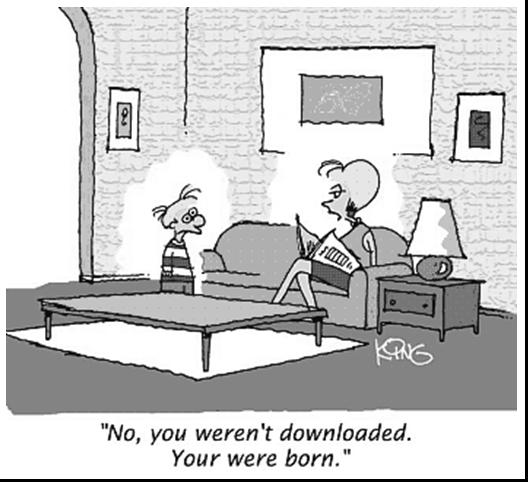
\includegraphics[width=.5\textwidth]{fig1.jpg}
\caption{A typical figure}
\label{fig:exampleFig1}
\end{figure}

\begin{figure}[ht]
\centering
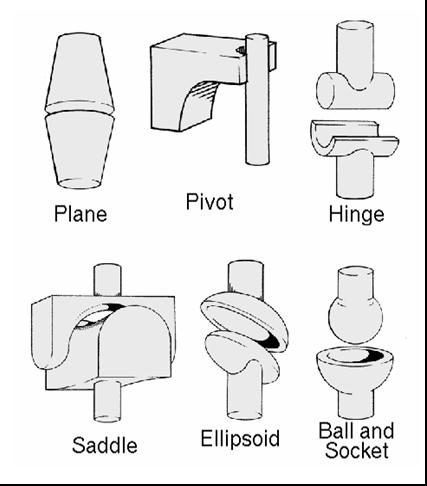
\includegraphics[width=.3\textwidth]{fig2.jpg}
\caption{This figure is an example of a figure caption taking more than one
  line and justified considering margins mentioned in Section~\ref{sec:figs}.}
\label{fig:exampleFig2}
\end{figure}

In tables, try to avoid the use of colored or shaded backgrounds, and avoid
thick, doubled, or unnecessary framing lines. When reporting empirical data,
do not use more decimal digits than warranted by their precision and
reproducibility. Table caption must be placed before the table (see Table 1)
and the font used must also be Helvetica, 10 point, boldface, with 6 points of
space before and after each caption.



\begin{thebibliography}{99}

\bibitem{belo2020} Belo, A. et al. (2020). Uma abordagem multi-período e bi-objetivo para alocação de ambulâncias em Belo Horizonte. *Revista de Pesquisa Operacional*.

\bibitem{bike2024} Silva, R. et al. (2024). Metaheurísticas aplicadas à localização de estações de bicicletas: estudo com algoritmos genéticos e simulated annealing. *Congresso Brasileiro de Computação*.

\bibitem{wikiLoc} Wikipedia. (2024). Facility location problem. Disponível em: \url{https://en.wikipedia.org/wiki/Facility_location_problem}. Acesso em: 2 set. 2025.

\end{thebibliography}

\end{document}
